\documentclass{ctexart}
\usepackage{graphicx}



\begin{document}
\title{OpenCL笔记整理}
\author{ }
\maketitle

\newpage
\section{模型}

\subsection{平台模型(Platform Model)}
OpenCL将所有计算机的硬件系统进行抽象,并提出以下硬件模型。并用这个模型代表所有的硬件系统。具体模型如下图所示:

\begin{figure}[!ht]
  \centering
  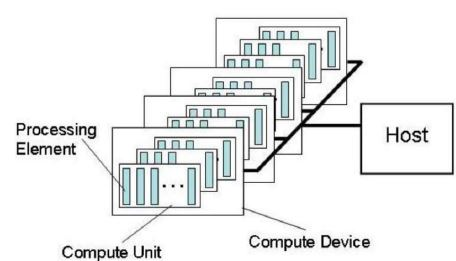
\includegraphics[width=0.7\linewidth]{yingjianceng.jpg}\\
  \caption{OpenCL硬件层模型}
\end{figure}
在实际的计算机系统中,Host 通常是一个CPU 担任,它负责为其他有计算功能的设备(device)分配任务;

而Compute Device代表计算设备,通常可以是GPU、CPU、DSP 等其他芯片。比如可以用一个CPU 作Host,而使用GPU 作为计算设备。

其中Processing Element 是上述芯片中的一个计算单元。比如对于一个CPU,可能是四核的,而Processing Element 可以代表其中一个核。

而Compute Unit是Processing Element 组成的组。通常,可以根据工作任务将Processing Element 分组,每一组称之为Compute Unit。 对于GPU或者FPGA 通常会将Processing Element 分组。

\subsection{内存模型(Memory Model)}
为了方便数据的存储和共享,OpenCL 将不同硬件平台上的内存结构,抽象成以下的内存模型。
\begin{figure}[!ht]
  \centering
  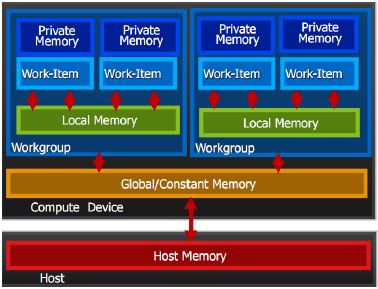
\includegraphics[width=0.6\linewidth]{neicunmoxing.jpg}\\
  \caption{OpenCL内存模型}
\end{figure}
对于Host一般负责任务的分配,所以会有自己的内存。

而Global/Constant Memory是Compute Device 的内存,其中数据所有计算单元(Processing Element)共享。比如如果计算设备是GPU,该内存就对应GPU 上的内存。

通常对于每个Processing Element (Work-Item)可能会附有私有内存(Private Memory),一般以缓存方式出现,其中数据由Processing Element 独享。

对于不同硬件平台,可能每一个组(Work Group)又会配有Local Memory,方便数据共享。

\subsection{执行模型(Execution Model)}
执行模型即是对编程过程中或运行过程中所用到的环境的抽象。
\begin{figure}[!ht]
  \centering
  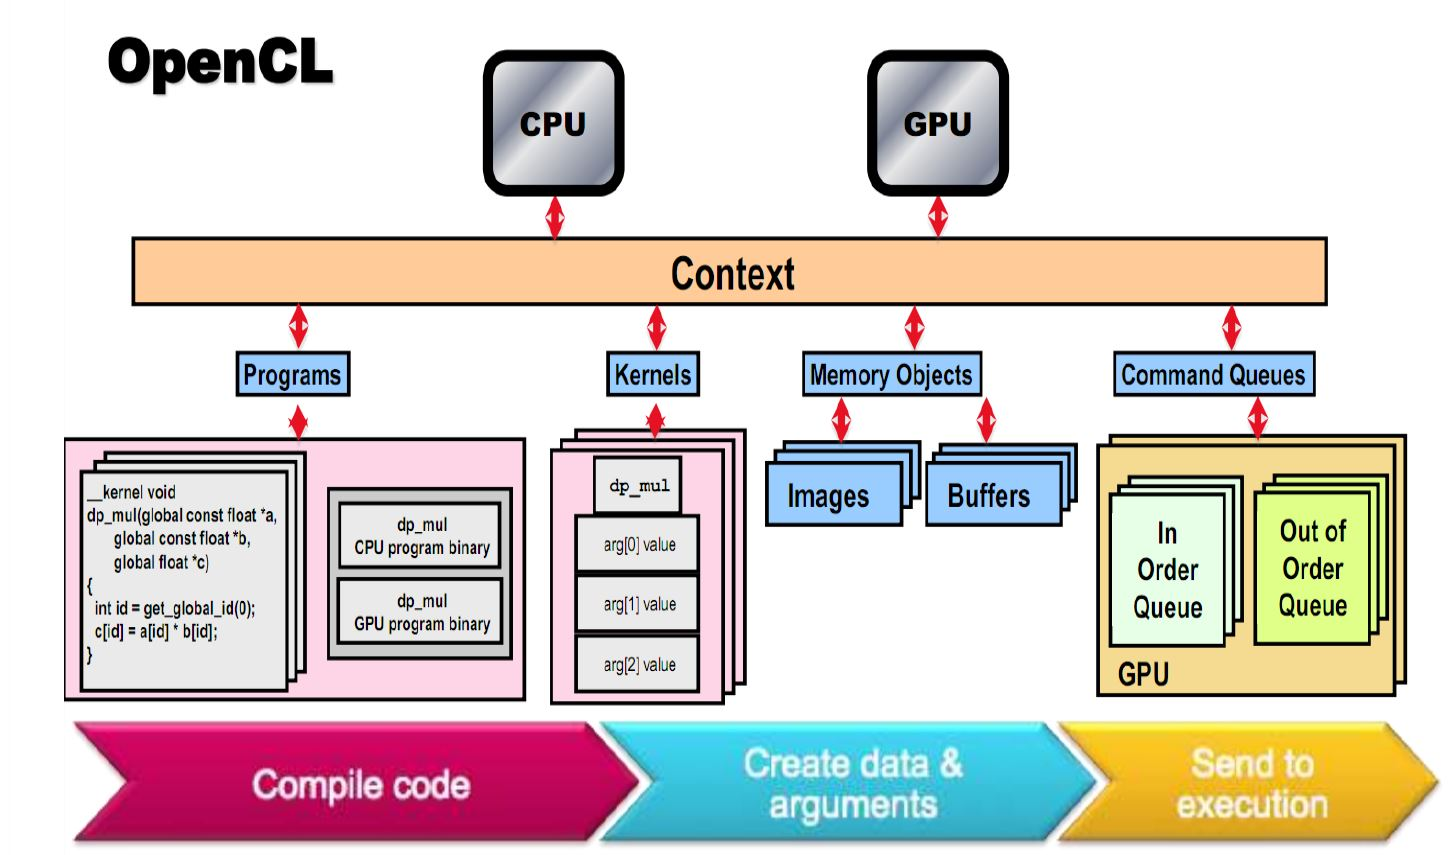
\includegraphics[width=0.7\linewidth]{ruanjianmoxing.jpg}\\
  \caption{OpenCL软件模型}
\end{figure}

执行模型在编程时可以分两部分,其中kernels 的代码在计算设备中运行;而host program 在host 中运行。

kernels需要在host配置的context环境内执行。该context 通常会含有:
\begin{description}
  \item[*devices]opencl 可用的计算设备
  \item[kernel objects] 可以在计算设备上运行的函数
  \item[program objects] 可以在kernel 上执行的源码
  \item[memory objects]host 和计算设备可以使用的数据。buffers:一块内存;images:多维内存
\end{description}

如上文所述,对于host program,需要配置context 环境给kernel 使用。host 使用command-queue 与计算设备进行协作。每一个command-queue 与一个计算设备对应。command 可以分为3 种:
\begin{description}
  \item[kernel-enqueue commands] 将命令入队的命令
  \item[memory commands] 数据交互的命令
  \item[synchronization commands]用于显式定义同步点
\end{description}




\newpage
\section{OpenCL编程}
流程:
\begin{enumerate}
  \item 确定并选择platforms\\
        相关函数:clGetPlatformIDs()/clGetPlatformInfo()
  \item 确定并选择devices\\
        相关函数:clGetDeviceIDs()/clGetDeviceInfo()
  \item 创建context\\
        相关函数:clCreateContext()
  \item 创建command queue\\
        相关函数:clCreateCommandQueue()
  \item 读写到device\\
        相关函数:clBuildProgram()/clCreateKernel()/clCreateBUffer()
  \item 启动kernel\\
        相关函数:clEnqueueNDRangeKernel()
  \item 释放资源(clean up)\\
        相关函数:clRelease*()
\end{enumerate}

\subsection{平台获取(platform)}
OpenCL最先要做的是获取平台信息。可以使用下述函数获取平台信息:
\begin{verbatim}
函数原型:
cl_int clGetPlatformIDs (cl_uint num_entries,  // 平台数
                         // 平台指针,返回找到的平台
                         cl_platform_id *platforms,
                         // 返回可用的平台数
                         cl_uint *num_platforms)
\end{verbatim}

\begin{verbatim}
调用样例:
// 获取当前可用平台数
cl_uint platform_number;
int status = clGetPlatformIDs(0, NULL, &platform_number);

// 根据可用平台数,分配空间
cl_platform_id* platforms
                    = new cl_platform_id[platform_number];

// 调用函数,获取platforms
status = clGetPlatformIDs(platform_number, platforms, NULL);
\end{verbatim}

\subsection{设备获取(device)}
当获取平台信息后,每个平台可能对应有多个设备,接下来要获取设备信息。设备类型分为CPU,GPU,ACCEGERATOR等,具体参考《The OpenCL Specification -version2.0》-table4.2
\begin{verbatim}
函数原型:
cl_int clGetDeviceIDs(cl_platform_id platform, // 平台信息
                      // 设备类型
                      cl_device_type device_type,
                      // 设备个数
                      cl_uint num_entries,
                      // 设备指针
                      cl_device_id *devices,
                      // 返回设备个数
                      cl_uint *num_devices)
\end{verbatim}

\begin{verbatim}
调用样例:
// 获取当前平台的设备
cl_uint device_number;
int status = clGetDeviceIDs(platform[0],
                            CL_DEVICE_TYPE_ALL,
                            0,
                            NULL,
                            &device_number);
// 根据可用平台数,分配空间
cl_device_id* devices
                    = new cl_device_id[device_number];

// 获取当前平台的设备数
status = clGetDeviceIDs(platform[0],
                        CL_DEVICE_TYPE_ALL,
                        device_number,
                        devices,
                        NULL);
\end{verbatim}

\subsection{配置context}
接下来需要给某个或多个设备配置相应的contex (环境),即配置相应的资源。以此管理诸如指令队列,内存,源码等信息。

\subsubsection{声明context对象}
\begin{verbatim}
函数原型:
cl_context clCreateContext(
            // context 特性及其对应的值
            const cl_context_properties *properties,
            // 设备个数
            cl_uint num_devices,
            // 设备指针
            const cl_device_id *devices,
            // 回调函数:当出现错误时自动调用
            void (CL_CALLBACK *pfn_notify)
                        (const char *errinfo,
                         const void *private_info,
                         size_t cb,
                         void *user_data),
            // 回调函数的参数
            void *user_data,
            // 返回的错误码
            cl_int *errcode_ret)
\end{verbatim}

其中context特性,可以指定与本context对应的平台以及OpenCL 和其他APIs的同步方式。

\begin{verbatim}
调用样例:
// 为第一个device配置contex
cl_context context = clCreateContext(
            NULL, 1, devices[0], NULL, NULL, NULL);
\end{verbatim}



\subsubsection{配置context 的指令队列(command queue)}
声明好context后,需要为其配置指令队列。这是一段内存空间,每个device 的指令都将先保存在这段内存中,再发送给device。
\begin{verbatim}
函数原型:
cl_command_queue clCreateCommandQueueWithProperties(
                        // 待配置的context
                        cl_context context,
                        // 声明context 时对应的设备
                        cl_device_id device,
                        // 指定指令队列的参数
                        const cl_queue_properties *properties,
                        // 返回的错误码
                        cl_int *errcode_ret)
\end{verbatim}

\begin{verbatim}
调用样例:
cl_command_queue command_queue =
        clCreateCommandQueue(context, devices[0], 0, NULL);
\end{verbatim}


\subsubsection{配置context 的源码对象(kernel object\&program object)}
\paragraph{创建源码对象}
由于异构计算的特殊性,这里需要载入在device中运行的源码并编译成可在异构平台执行的文件。所有操作通过调用相应的函数实现。


\subparagraph{编写kernel.cl}就是在device中实际运行的代码。这段代码可以以字符串的形式写在源文件中,也可以单独写成一个.cl 文件。其具体格式与一个C/C++函数类似,只是变量之前要注明限定符。

\begin{verbatim}
代码举例:
// 这段代码将会并行执行
__kernel void func(
        __global const float* a,  // 数组a
        __global const float* b,  // 数组b
        __global float* c) // 数组c,存放结果
{
    int id = get_global_id(0); // 获取运算单元id
    c[id] = a[id] + b[id];  // 计算结果
}
\end{verbatim}


\subparagraph{字符串格式的.cl}如果是以字符串的形式写在源文件中,每行用一个字符串表示,并且要注意换行需要使用转义字符,比如:
\begin{verbatim}
代码举例:
const char *source =
        "__kernel void memset( __global uint *dst ) \n"
        "{ \n"
        " dst[get_global_id(0)] = get_global_id(0); \n"
        "} \n";
\end{verbatim}


\subparagraph{源码对象的创建}
声明program对象可以使用以下函数:
\begin{verbatim}
函数原型:
cl_program clCreateProgramWithSource(
                            // 指定对应的context
                            cl_context context,
                            // 二维字符串数组的个数
                            cl_uint count,
                            // 字符串
                            const char **strings,
                            // 字符串长度的数组
                            const size_t *lengths,
                            // 错误码
                            cl_int *errcode_ret)

cl_program clCreateProgramWithBuiltInKernels(
                            cl_context context,
                            cl_uint num_devices,
                            const cl_device_id *device_list,
                            const char *kernel_names,
                            cl_int *errcode_ret)
\end{verbatim}

其中关于字符串长度的数组,可以设置为NULL,但要求字符串以结束符结尾。否则,要根据实际请设置其中数值。
\begin{verbatim}
调用样例:
cl_program program =
    clCreateProgramWithSource(context,
                              1, // 字符串数组的个数
                              &source, // 字符串数组头
                              NULL, NULL);
\end{verbatim}


\paragraph{编译并链接源码}
上文载入源码后,调用本函数进行编译并链接。

(builds = compiles + links)。
\begin{verbatim}
函数原型:
cl_int clBuildProgram(cl_program program, // program对象
                      cl_uint num_devices, // 设备个数
                      // 设备指针
                      const cl_device_id *device_list,
                      // 编译选项字符串
                      const char *options,
                      // 回调函数:build之后自动调用
                      void (CL_CALLBACK *pfn_notify)
                                (cl_program program,
                                void *user_data),
                      // 回调函数参数
                      void *user_data)
\end{verbatim}

\subsubsection{配置context 的内存对象(memory objects)}
\begin{verbatim}
函数原型:
cl_mem clCreateBuffer(cl_context context, // context对象
                      cl_mem_flags flags, // 内存模型
                      size_t size, // 内存大小(bytes)
                      void *host_ptr, // 内存指针
                      cl_int *errcode_ret) // 错误码
\end{verbatim}
其中flags具体可参考《The OpenCL Specification -version2.0》-table5.3


\begin{verbatim}
调用样例:
cl_mem buffer = clCreateBuffer(
        context,
        // 输入内存为只读,并可以从宿主机内存复制到设备内存
        CL_MEM_READ_ONLY | CL_MEM_COPY_HOST_PTR,
        // 输入内存空间大小(N个int的大小)
        N * sizeof(int),		
        (void *)buffer_pointer,
        NULL);
\end{verbatim}

根据table5.3中内容,上述CL\_MEM\_COPY\_HOST\_PTR表示,本函数分配的内存使用buffer\_pointer指向的内容初始化,先分配内存再将指针内容拷贝过去。

根据实际需求,可多次调用上述函数,分配多块内存方便使用。通常可以分配一块输入内存,一块输出内存,分别用于数据的输入(从host--device),和输出。

\subsection{配置kernel}

\paragraph{声明kernel对象}
\begin{verbatim}
函数原型:
cl_kernel clCreateKernel(cl_program program, // program对象
                         // kernel.cl中的函数名
                         const char *kernel_name,
                         cl_int *errcode_ret)
\end{verbatim}


\paragraph{配置kernel对象参数}
即kernel函数的参数,需要调用此函数进行传输。
\begin{verbatim}
函数原型:
cl_int clSetKernelArg(cl_kernel kernel, // kernel指针
                      cl_uint arg_index, // 参数下标,[0,n-1]
                      size_t arg_size, // 参数尺寸
                      const void *arg_value)
\end{verbatim}

kernel函数有几个参数,就需要调用几次上述函数。其中参数下标从0开始,一直到n-1。

比如输入参数为上面声明内存对象时,代码举例中的内存对象“buffer”:
\begin{verbatim}
调用样例:
cl_int status = clSetKernelArg(kernel,
                        	   0,		// 参数索引
                        	   sizeof(cl_mem), // 参数尺寸
                        	   (void *)&buffer); // 参数指针
\end{verbatim}


\subsection{运行kernel}

调用下面的函数,使命令入队。
\begin{verbatim}
函数原型:
cl_int clEnqueueNDRangeKernel(
                        // 指令队列对象
                        cl_command_queue command_queue,
                        // kernel对象
                        cl_kernel kernel,
                        // 工作维度:1,2,3维
                        cl_uint work_dim,
                        // 指定各个维度上的起始id。默认为0
                        const size_t *global_work_offset,
                        // 各个维度的尺寸
                        const size_t *global_work_size,
                        const size_t *local_work_size,
                        // 指定需要先完成的操作(对象)
                        cl_uint num_events_in_wait_list,
                        const cl_event *event_wait_list,
                        // 返回事件对象
                        cl_event *event)
\end{verbatim}



\subsection{读取结果}
该操作为读(写)操作,与上述分配内存对象不同。在kernel运行时,可以根据需要读写内存(读写速度可能较慢)。
\begin{verbatim}
函数原型:
cl_int clEnqueueReadBuffer (
                        // 指令队列对象
                        cl_command_queue command_queue,
                        // 内存对象,用clCreateBuffer()声明
                        cl_mem buffer,
                        // true:内存读取结束之前,函数不返回
                        // false: 将读取命令入队后即返回
                        cl_bool blocking_read,
                        // 内存读(写)的起始,和尺寸
                        size_t offset,
                        size_t size,
                        // 内存指针,内存读取后,复制到此
                        void *ptr,
                         // 指定需要先完成的操作(对象)
                        cl_uint num_events_in_wait_list,
                        const cl_event *event_wait_list,
                        // 返回事件对象
                        cl_event *event)


cl_int clEnqueueWriteBuffer (
                        // 指令队列对象
                        cl_command_queue command_queue,
                        // 内存对象,用clCreateBuffer()声明
                        cl_mem buffer,
                        // true:内存读取结束之前,函数不返回
                        // false: 将读取命令入队后即返回
                        cl_bool blocking_read,
                        // 内存读(写)的起始,和尺寸
                        size_t offset,
                        size_t size,
                        // 内存指针,与内存对象声明时一致
                        void *ptr,
                         // 指定需要先完成的操作(对象)
                        cl_uint num_events_in_wait_list,
                        const cl_event *event_wait_list,
                        // 返回事件对象
                        cl_event *event)
\end{verbatim}

\begin{verbatim}
调用举例:
cl_int status = clEnqueueReadBuffer(
                // 命令队列
                command_queue,	
                // 输出内存对象	
                buffer,	
                // 内核读取结束之前该函数不会返回
                CL_TRUE,			
                0, // 起始位置偏移
                N * sizeof(int), // 内存尺寸,这里为举例
                // 内存指针
                buffer_pointer,
                0,
                NULL,
                NULL);
\end{verbatim}


\subsection{释放资源}
这里需要释放掉上述过程中声明的对象,具体函数原型省略。除了释放OpenCL的对象,也需要释放使用new声明的内存空间,防止内存泄漏。
\begin{verbatim}
调用举例:
status = clReleaseKernel(kernel);
status = clReleaseProgram(program);
status = clReleaseMemObject(buffer);
status = clReleaseCommandQueue(command_queue);
status = clReleaseContext(context);
\end{verbatim}


\newpage
\section{代码举例}
\begin{verbatim}
#include <CL/cl.h>
#include <stdio.h>
#define NWITEMS 512

// 一个kernel代码,举例。
const char *source =
        "__kernel void memset( __global uint *dst ) \n"
        "{ \n"
        " dst[get_global_id(0)] = get_global_id(0); \n"
        "} \n";


int main(int argc, char ** argv)
{
// 1. 获取平台
cl_platform_id platform;
clGetPlatformIDs( 1, &platform, NULL );

// 2. 获取设备.
cl_device_id device;
clGetDeviceIDs( platform, CL_DEVICE_TYPE_GPU,
                1,
                &device,
                NULL);

// 3. 创建context
cl_context context = clCreateContext( NULL,
                                      1,
                                      &device,
                                      NULL, NULL, NULL);
// 4.创建comand queue
cl_command_queue queue = clCreateCommandQueue( context,
                                               device,
                                               0, NULL );

// 4. 读入kernel代码,创建kernel,创建buffer
cl_program program = clCreateProgramWithSource( context,
                                                1,
                                                &source,
                                                NULL, NULL );
clBuildProgram( program, 1, &device, NULL, NULL, NULL );
cl_kernel kernel = clCreateKernel( program, "memset", NULL );

cl_mem buffer = clCreateBuffer( context,
                                CL_MEM_WRITE_ONLY,
                                NWITEMS * sizeof(cl_uint),
                                NULL, NULL );

// 6. 启动kernel.
size_t global_work_size = NWITEMS;
clSetKernelArg(kernel, 0, sizeof(buffer), (void*) &buffer);
clEnqueueNDRangeKernel( queue,
                        kernel,
                        1,
                        NULL,
                        &global_work_size,
                        NULL, 0, NULL, NULL);
clFinish( queue );

// 7. 读取结果
cl_uint *ptr;
ptr = (cl_uint *) clEnqueueMapBuffer( queue,
                                      buffer,
                                      CL_TRUE,
                                      CL_MAP_READ,
                                      0,
NWITEMS * sizeof(cl_uint),
                                      0, NULL, NULL, NULL );
int i;
for(i=0; i < NWITEMS; i++)
    printf("%d %d\n", i, ptr[i]);

// 8.自动释放资源或手动释放,例如:
//clReleaseKernel(kernel);
//clReleaseProgram(program);
// ...

return 0;
}
\end{verbatim}



\section{关于执行模型(execution model)}
如之前所述,执行模型可以分为两部分:kernel和host program两部分。其中kernel和实际计算设备相对应。

在配置kernel时,需要配置一个context对象。

context中的command\_queue对象传递给device需要经过以下几个过程:
\begin{enumerate}
  \item 入队(queued)
  \item 传递(submitted)
  \item 就绪(ready)命令被存放在device的work-pool中,准备被调度
  \item 运行(running)与该命令相关联的work-groups会执行该命令
  \item 结束(ended)
  \item 完成(complete)
\end{enumerate}



\end{document}
